\subsection*{The separation framework}
We describe a general approach for reducing parity games to safety games.
\Cref{1-sec:reductions} constructs reductions between objectives using automata: 
in the case at hand parity reduces to safety if there exists a deterministic automaton $\Automaton$ over the alphabet $[1,d]$
with acceptance objective $\Safe$ and defining $\Parity([1,d])$,
meaning $L(\Automaton) = \Parity([1,d])$.
With such an automaton in hand~\cref{1-lem:automata_reduction} implies the following reduction:
from a parity game $\game$ construct the safety game $\game \times \Automaton$ satisfying that
Eve has a winning strategy in $\Game$ from $v_0$ if and only if she has a winning strategy in $\Game \times \Automaton$ from $(v_0,q_0)$.

\vskip1em
Unfortunately, it can be shown (using a topological argument) that there is no such automaton.
The separation framework defines a (weaker) sufficient condition for the reduction above to be correct.
Instead of insisting that $L(\Automaton) = \Parity([1,d])$,
it is enough to have $\WE(\arena,\Parity[\col]) = \WE(\arena,L(\Automaton)[\col])$.
To ensure this equality we will only require that $L(\Automaton)$ \textit{separates} winning plays from losing plays.
The two \textit{key} ideas are first to take advantage of the positionality of parity objectives 
by restricting further winning plays to \textit{positional} winning plays,
and second to state $\WE(\arena,\Parity[\col]) = \WE(\arena,L(\Automaton)[\col])$ not for all parity games,
but only for parity games with $n$ vertices and priorities in $[1,d]$.

\vskip1em
A deterministic safety automaton over the alphabet $[1,d]$ is given by 
\[
\Automaton = (Q,q_0,\delta : Q \times [1,d] \to Q,\Safe[\col_\Automaton]),
\]
where $\col_\Automaton : Q \times [1,d] \to \set{\Win,\Lose}$.
A word $w \in [1,d]^\omega$ is accepted if the run $\rho$ over $w$ only contains transitions in $\Win$.
We use the following simplifying convention for safety automata: we distinguish a special rejecting state $\bot$
and assume that all transitions are accepting except the ones leading to $\bot$. 
Said differently, a word $w$ is accepted if and only if it the run over $w$ does not contain the state $\bot$.
Hence we do not need to specify $\col_\Automaton$:
in the next two sections by an automaton we mean a deterministic safety automaton
given by $\Automaton = (Q,q_0,\delta : Q \times [1,d] \to Q)$.

\vskip1em
Let us now give a sufficient condition for the automaton $\Automaton$ 
to imply the correctness of the reduction from the parity game $\Game$ to the safety game $\Game \times \Automaton$.
The condition that we define now is that the automaton $\Automaton$ is $(n,d)$-separating; it relies on the notion of parity graphs.
Recall a parity graph ""satisfies"" parity from $v$ if all infinite paths from $v$ satisfy parity,
and that a strategy $\sigma$ is winning from $v$ if and only if the parity graph $\Game[\sigma]$ satisfies parity from $v$.

We say that an automaton reads, accepts, or rejects a path $\pi$ in a parity graph, 
which is an abuse because what the automaton reads is the induced sequence of colours $\col(\pi)$.

\begin{definition}[Separating automata]
\label{3-def:separating_automata}
An automaton $\Automaton$ is $(n,d)$-\textit{separating} if the two following properties hold.
\begin{itemize}
	\item For all parity graphs $G$ with $n$ vertices and priorities in $[1,d]$ satisfying parity from $v$, 
	all paths from $v$ are accepted by $\Automaton$.
	
	\item All words accepted by $\Automaton$ satisfy parity.
\end{itemize}
\end{definition}
We define the objective $\Parity_{\mid n}$ over the set of colours $[1,d]$ as:
\[
\Parity_{\mid n} = 
\set{ \play : 
\begin{array}{l}
\play \text{ is a path starting from some vertex $v$ in some parity graph} \\
\text{with } n \text{ vertices and priorities in } [1,d] \text{ satisfying } \Parity \text{ from } v
\end{array}}.
\]
%For a parity graph $G$ and a vertex $v$, we let $\Paths(G,v) \subseteq [1,d]^\omega$ denote the set of infinite paths from $v$.
%We define the objective $\Parity_{\mid n}$ over the set of colours $[1,d]$ as:
%\[
%\Parity_{\mid n} = \bigcup \set{ \Paths(G,v) : 
%\begin{array}{l}
%G \text{ parity graph with } n \text{ vertices and priorities in } [1,d] \\
%\text{ satisfying } \Parity \text{ from } v
%\end{array}}.
%\]
The definition of $(n,d)$-separating automata is illustrated in \cref{3-fig:separation} and can be summarised
as $\Parity_{\mid n} \subseteq L(\Automaton) \subseteq \Parity$.

\begin{figure}[!ht]
\centering
  \begin{tikzpicture}
    \begin{scope}
      \draw[clip,use as bounding box] (0,0) ellipse (2cm and 1.2cm);
      \draw[dgrey] (0,0) ellipse (2cm and 1.2cm);
      \draw[white] (-2,0) ellipse (2.9cm and 2.5cm);
      \draw[lgrey] (-2,0) ellipse (1.5cm and 1.3cm);
      \draw[hatcharea,hatchspread=6pt] (-2,0) ellipse (2.1cm and 1.7cm);
      \draw (0,0) ellipse (2cm and 1.2cm);
    \end{scope}
    \path[arrow]
      (2.2,1.6) node[] {$[1,d]^\omega \setminus$ \textsf{Parity}} edge (1.5,.3)
      (0,1.6) node[] {\textsf{Parity}} edge (.4,.5)
      (-2,1.6) node[] {\textsf{Parity}$_{|n}$} edge (-1.4,.2)
      (-1.5,-1.5) node[below,anchor=base] {$L(\Automaton)$} edge (-.4,-.6);
  \end{tikzpicture}
\caption{The separation problem.}
\label{3-fig:separation}
\end{figure}

The following lemma shows the definition of separating automata in action.

\begin{lemma}[Game equivalence using separating automata]
\label{3-lem:separating_automata}
Let $\Automaton$ an $(n,d)$-separating automaton.
Then for all parity games $\game = (\arena,\Parity[\col])$ with $n$ vertices and priorities in $[1,d]$, 
we have
\[
\WE(\game) = \WE(\arena,L(\Automaton)[\col]).
\]
\end{lemma}

\begin{proof}
The inclusion $\WE(\game) \subseteq \WE(\arena,L(\Automaton)[\col])$ follows from positional determinacy and the inclusion 
$\Parity_{\mid n} \subseteq L(\Automaton)$.
Let $v \in \WE(\game)$.
Consider $\sigma$ a positional strategy ensuring parity from $v$ and construct the parity graph $\game[\sigma]$, it satisfies parity from $v$.
Hence the strategy $\sigma$ also ensures $L(\Automaton)[\col]$ from $v$, so $v \in \WE(\arena,L(\Automaton)[\col])$.

Conversely, the inclusion $L(\Automaton) \subseteq \Parity$ implies the inclusion 
$L(\Automaton)[\col] \subseteq \Parity[\col]$, which in turn implies 
$\WE(\arena,L(\Automaton)[\col]) \subseteq \WE(\game)$.
\end{proof}

The last step is to explain how to solve a game with objective $L(\Automaton)$, as already discussed in~\cref{1-sec:reductions}.
Let $\Game = (\arena, L(\Automaton)[\col])$.
We construct a safety game by making the synchronised product of the arena with the automaton:
\[
\Game \times \Automaton = (\arena \times \Automaton, \Safe[\col']),
\]
where the safety condition ensures that the play is accepted by $\Automaton$.
Formally, we construct the arena $\arena \times \Automaton$ as follows.
We first define the graph $G \times Q$ whose set of vertices is $V \times Q$ and set of edges is defined as follows:
for every edge $(v,v') \in E$ and state $q \in Q$ there is an edge from $(v,q)$ to $(v',\delta(q,\col(u)))$.
The arena is $\arena \times \Automaton = (G \times Q, \VE \times Q, \VA \times Q)$.
Using the convention for safety automata that the rejecting transitions are precisely those leading to the rejecting state $\bot$,
the colouring function is defined by $\col'(v,q) = \Win$ if $q \neq \bot$, and $\Lose$ otherwise.

\begin{fact}[Reduction to safety games using separating automata]
\label{3-fact:reduction}
Eve has a winning strategy in $\game$ from $v_0$ if and only if
she has a winning strategy in $\Game \times \Automaton$ from $(v_0,q_0)$.
\end{fact}

\begin{theorem}[Algorithm using separating automata]
\label{3-thm:algorithm_separating_automata}
Let $\Automaton$ an $(n,d)$-separating automaton.
There exists an algorithm for solving parity games of complexity $O(m \cdot |\Automaton|)$.
\end{theorem}
\begin{proof}
Let $\Game$ a parity game with $n$ vertices and priorities in $[1,d]$.
Thanks to~\cref{3-lem:separating_automata} and \cref{3-fact:reduction}, solving $\Game$
is equivalent to solving the safety game $\Game \times \Automaton$.
Thanks to~\cref{2-thm:reachability} solving safety games can be done in time linear in the number of edges.
This yields an algorithm for solving parity games whose running time is $O(m \cdot |\Automaton|)$.
\end{proof}

In the remainder of this section we give a construction for a quasipolynomial $(n,d)$-separating automaton.

\subsection*{The original separating automaton}
\begin{theorem}[The original separating automaton]
\label{3-thm:original_separating_automaton}
There exists an $(n,d)$-separating automaton of size $n^{O(\log d)}$,
inducing an algorithm for solving parity games of complexity $n^{O(\log d)}$.
\end{theorem}

\paragraph{\bf $i$-sequences.}
The key definition used by the original separating automaton is an
\emph{$i$-sequence}. Let $\pi = p_1, p_2, \dots, p_t$ a finite sequence of
priorities. An $i$-sequence is a set of \emph{indices} that splits $\pi$ into
sub-sequences. An $i$-sequence consists of exactly $2^i$ indices $1 \le j_1 <
j_2 < \dots < j_{2^i} \le t$, where each $j_k$ is an integer that refers to the
priority $p_{j_k}$ from the sequence $\pi$. An $i$-sequence is required to
satisfy the following properties. 
\begin{itemize} \item \textbf{Evenness.} Each
index (except possibly the last index) refers to an even priority, meaning that
$p_{j_k}$ is an even priority for all $k < 2^i$.

\item \textbf{Inner domination.} The subsequence of priorities between any two
indices $j_k$ and $j_{k+1}$ is dominated by either $p_{j_k}$ or $p_{j_{k+1}}$.
Formally, this means that whenever $j_k < l < j_{k+1}$, we have that $p_l \le
p_{j_k}$ or we have that $p_l \le p_{j_{k+1}}$.

\item \textbf{Outer domination.} The final subsequence between $p_{j_{2^i}}$ and
$p_t$ is dominated by $p_{j_{2^i}}$, meaning that for all $l > j_{2^i}$ we have
$p_l \le p_{j_{2^i}}$.
\end{itemize}

\begin{figure}[!ht]
    \begin{center}
    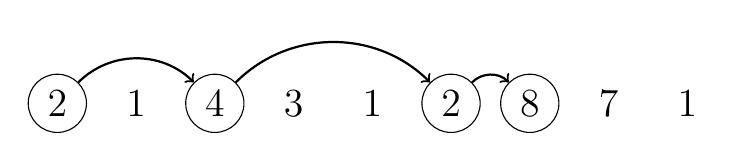
\begin{tikzpicture}

    \tikzstyle{seqc}=[draw, circle]

    \node [seqc] (1) {\Large $2$};
    \node [right of=1, node distance=1cm] (2) {\Large $1$};
    \node [seqc, right of=2, node distance=1cm] (3) {\Large $4$};
    \node [right of=3, node distance=1cm] (4) {\Large $3$};
    \node [right of=4, node distance=1cm] (5) {\Large $1$};
    \node [seqc, right of=5, node distance=1cm] (6) {\Large $2$};
    \node [seqc, right of=6, node distance=1cm] (7) {\Large $8$};
    \node [right of=7, node distance=1cm] (8) {\Large $7$};
    \node [right of=8, node distance=1cm] (9) {\Large $1$};

    \path[->,thick,bend left=45]
        (1) edge (3)
        (3) edge (6)
        (6) edge (7)
        ;
    \end{tikzpicture}
    \end{center}
    \caption{A $2$-sequence.}
\label{3-fig:isequence}
\end{figure}

\Cref{3-fig:isequence} gives an example of a $2$-sequence. The circled
priorities are the indices used in the sequence. Note that there are exactly
$2^2 = 4$ indices used, and that every circled priority is even. Inner
domination is satisfied because every priority that is between two circled
priorities is lower than one of the two end points, and outer domination is
satisfied because the final circled priority $8$ is larger than all the
priorities that come after it.

\paragraph{\bf The relationship to parity games.}
The relationship between $i$-sequences and parity games is explained by the
following lemma.

\begin{lemma}[Completeness for the separating automaton]
\label{3-lem:isequencewin}
Suppose that Adam and Eve play positional strategies in the parity game,
and let $\pi$ the resulting play.
\begin{itemize}
\item If Eve wins the parity game, then there exists prefixes of $\pi$ that
contain arbitrarily long $i$-sequences.
\item If Adam wins the parity game, then no prefix of $\pi$ will contain a
$\lceil \log n \rceil$-sequence.
\end{itemize}
\end{lemma}
\begin{proof}
If Eve wins the parity game then the largest
priority occurring in $\pi$ infinitely often is even. Let $p$ this priority.
To construct a prefix containing an $i$-sequence, we find the first index $j$
after which no priority $q > p$ is seen. We take as our indices $j_1 < j_2 <
\dots < j_{2^i}$ the first $2^i$ occurrences of priority $p$ after index $j$.
Evenness is trivially satisfied, and both inner and outer domination are
satisfied because no priority larger than $p$ is seen after index $j$.

We prove the second claim by contradiction. Suppose that Adam wins the game, but
that there is a prefix of $\pi$ that contains a $\lceil \log n \rceil$-sequence.
Since the sequence indexes $2^{\lceil \log n \rceil} \ge n$ vertices of the
game, it must index the same vertex $v$ twice. Thus our $i$-sequence must
contain a cycle passing through $v$. Note that inner domination ensures that the
largest priority on the cycle that passes through $v$ is even. However, no even
cycle can be formed when Adam wins the game by playing a positional winning
strategy, and so we have arrived at our contradiction.
\end{proof}

To summarise, if Eve wins the game, then she has a strategy that ensures that
arbitrarily long $i$-sequences occur, while if Adam wins the game then he has a
strategy that ensures that no $\lceil \log n \rceil$-sequence occurs. So to
solve the parity game, it is sufficient to determine whether Eve can force a
$\lceil \log n \rceil$-sequence to occur.

\paragraph{\bf A data structure for recognising $i$-sequences.}
We will build a quasi-polynomial sized automaton that reads a sequence of
priorities, 
and determines whether that sequence of priorities contains a
$k$-sequence. 
The automaton is defined by a data structure that we call a \emph{record}, which
contains information about the $i$-sequences that have been seen so far in the
sequence.  

A record is a sequence $b_k, b_{k-1}, \dots, b_1, b_0$, where each
$b_i$ is either a priority, or the special symbol $\siblank$. The value of $b_i$
has the following meaning: 
\begin{itemize}
\item \textbf{Witnessing.} If $b_i \ne \siblank$, then we have seen an
$i$-sequence, and the final priority on that $i$-sequence is $b_i$. 
\item \textbf{Order.} If $b_i \ne \siblank$ and $b_j \ne \siblank$ and $j < i$,
then the first index of the $j$-sequence witnessed by $b_j$ occurs after the
last index of the $i$-sequence witnessed by $b_i$.
\end{itemize}
Note that, although each element $b_i$ records the existence of an
$i$-sequence, the record data structure \emph{does not} store the $2^i$ indices
of this $i$-sequence, it only stores the priority of the final index of that
sequence.

\begin{figure}[!ht]
    \begin{center}
    \begin{tikzpicture}
    \tikzstyle{seqc}=[draw, circle]
    \node [seqc,red] (1) {\Large $2$};
    \node [right of=1, node distance=0.9cm] (2) {\Large $1$};
    \node [seqc, red, right of=2, node distance=0.9cm] (3) {\Large $4$};
    \node [seqc, red, right of=3, node distance=0.9cm] (4) {\Large $2$};
    \node [seqc, red, right of=4, node distance=0.9cm] (5) {\Large $8$};
    \node [right of=5, node distance=0.9cm] (6) {\Large $7$};
    \node [seqc, blue, right of=6, node distance=0.9cm] (7) {\Large $2$};
    \node [right of=7, node distance=0.9cm] (8) {\Large $1$};
    \node [seqc, blue, right of=8, node distance=0.9cm] (9) {\Large $4$};
    \node [right of=9, node distance=0.9cm] (10) {\Large $1$};
    \node [seqc, grey, right of=10, node distance=0.9cm] (11) {\Large $2$};

    \path[->,thick,bend left=45,red]
        (1) edge (3)
        (3) edge (4)
        (4) edge (5)
        ;

    \path[->,thick,bend left=45,blue]
        (7) edge (9)
        ;
    \end{tikzpicture}
    \end{center}
\caption{An example sequence that corresponds to the record $\siblank 8 4 2$.}
\label{3-fig:ds}
\end{figure}

\Cref{3-fig:ds} shows an example sequence that is consistent with the
record that sets $b_3 = \siblank$, $b_2 = 8$, $b_1 = 4$, and $b_0 = 2$.
The red $2$-sequence is represented by $b_2 = 8$, which is the last priority of
the $2$-sequence. The blue $1$-sequence starts after the end of the
$2$-sequence, and it is represented by $b_1 = 4$. Likewise the grey
$0$-sequence starts after the end of the $1$-sequence, and is represented by
$b_0 = 2$. There is no $3$-sequence in the example, and this is represented by
setting $b_3 = \siblank$.

\paragraph{\bf The update rule.}
Suppose that we have a record that represents the $i$-sequences in a
finite sequence of priorities, and that we then read the next priority $p$ in
that sequence. We need to update the record to take this priority into
account. We do this by applying the following \emph{update rule}.
The update rule consists of two steps, which occur one after the other.

\begin{itemize}
\item \textbf{Step 1.} In this step, we find the largest index $i$
such that $b_j$ is even for all $j \le i$. If $b_i = \siblank$, or $b_i < p$,
then we create a new record $b'_k$, $b'_{k-1}$, \dots, $b'_0$ by
setting:
\begin{equation*}
b'_j = \begin{cases}
b_j & \text{if $j > i$,} \\
p & \text{if $j = i$,} \\
\siblank & \text{if $j < i$.} 
\end{cases}
\end{equation*}
If there is no index $i$ that satisfies the conditions, then we do not modify
the record.

\item \textbf{Step 2.} In step 2, we take the output of step 1, and we find the
largest index $i$ such that $p > b_i$ and we create a new record $b'_k$,
$b'_{k-1}$, \dots, $b'_0$ by setting:
\begin{equation*}
b'_j = \begin{cases}
b_j & \text{if $j > i$,} \\
p & \text{if $j = i$,} \\
\siblank & \text{if $j < i$.} 
\end{cases}
\end{equation*}
Again, if there is no such index $i$, then the record is not modified.
\end{itemize}

\begin{figure}[!ht]
    \begin{center}
    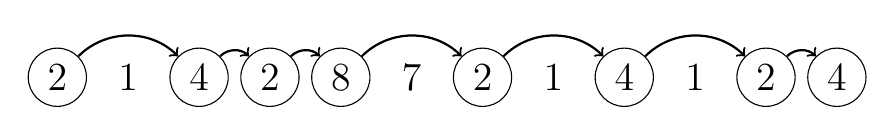
\begin{tikzpicture}
    \tikzstyle{seqc}=[draw, circle]
    \node [seqc] (1) {\Large $2$};
    \node [right of=1, node distance=0.9cm] (2) {\Large $1$};
    \node [seqc, right of=2, node distance=0.9cm] (3) {\Large $4$};
    \node [seqc, right of=3, node distance=0.9cm] (4) {\Large $2$};
    \node [seqc, right of=4, node distance=0.9cm] (5) {\Large $8$};
    \node [right of=5, node distance=0.9cm] (6) {\Large $7$};
    \node [seqc, right of=6, node distance=0.9cm] (7) {\Large $2$};
    \node [right of=7, node distance=0.9cm] (8) {\Large $1$};
    \node [seqc, right of=8, node distance=0.9cm] (9) {\Large $4$};
    \node [right of=9, node distance=0.9cm] (10) {\Large $1$};
    \node [seqc, right of=10, node distance=0.9cm] (11) {\Large $2$};
    \node [seqc, right of=11, node distance=0.9cm] (12) {\Large $4$};
    %\onslide<5>{\node [seq, right of=11, node distance=0.9cm] (12) {\Large
    %$\mathbf{9}$};}

    \path[->,thick,bend left=45]
        (1) edge (3)
        (3) edge (4)
        (4) edge (5)
        (5) edge (7)
        (7) edge (9)
        (9) edge (11)
        (11) edge (12)
        ;

    \end{tikzpicture}
    \end{center}
    \caption{An example of a Step 1 update applied to the sequence and record from~\cref{3-fig:ds}}
\label{3-fig:ds1}
\end{figure}
Intuitively, Step 1 attempts to combine the $i$-sequences in the existing record
into a longer $i$-sequence. Suppose that we have read the sequence shown in~\cref{3-fig:ds}, 
that we have compute the record $\siblank 8 4 2$, and that the next priority in the sequence is $4$.
\Cref{3-fig:ds1} shows the result of applying Step 1 to this situation.
Observe that $3$ is the largest index $i$ such that for all $j < i$ we have that
$b_j$ is even, so Step 1 will output the record $4 \siblank \siblank \siblank$.

So in this circumstance, Step 1 claims that we have now seen a $3$-sequence.
\Cref{3-fig:ds1} shows why this is correct: the $0$-sequence of $b_0$, the
$1$-sequence of $b_1$, and the $2$-sequence of $b_2$ can be merged together,
along with the new priority, to create a $3$-sequence. Observe that inner
domination in this new $3$-sequence is satisfied due to the outer domination
property for each of the $i$-sequences that it was constructed from.
For example, the $2$-sequence ends at priority $8$, and the $1$-sequence begins
at priority $2$, and we know that $8$ must dominate all priorities between the
$8$ and the $2$ because $8$ is required to dominate \emph{all} priorities that
follow it.

\begin{figure}[!ht]
    \begin{center}
    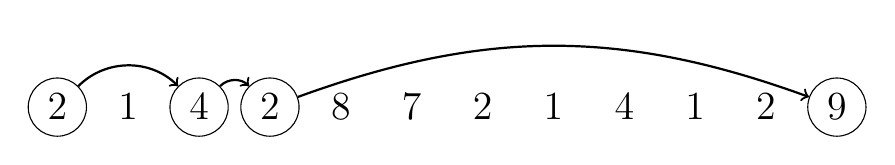
\begin{tikzpicture}
    \tikzstyle{seqc}=[draw, circle]
    \node [seqc] (1) {\Large $2$};
    \node [right of=1, node distance=0.9cm] (2) {\Large $1$};
    \node [seqc, right of=2, node distance=0.9cm] (3) {\Large $4$};
    \node [seqc, right of=3, node distance=0.9cm] (4) {\Large $2$};
    \node [right of=4, node distance=0.9cm] (5) {\Large $8$};
    \node [right of=5, node distance=0.9cm] (6) {\Large $7$};
    \node [right of=6, node distance=0.9cm] (7) {\Large $2$};
    \node [right of=7, node distance=0.9cm] (8) {\Large $1$};
    \node [right of=8, node distance=0.9cm] (9) {\Large $4$};
    \node [right of=9, node distance=0.9cm] (10) {\Large $1$};
    \node [right of=10, node distance=0.9cm] (11) {\Large $2$};
    \node [seqc, right of=11, node distance=0.9cm] (12) {\Large $9$};
    %\onslide<5>{\node [seq, right of=11, node distance=0.9cm] (12) {\Large
    %$\mathbf{9}$};}

    \path[->,thick,bend left=45]
        (1) edge (3)
        (3) edge (4);

    \path[->,thick,bend left=20]
        (4) edge (12)
        %(5) edge (7)
        %(7) edge (9)
        %(9) edge (11)
        %(11) edge (12)
        ;

    \end{tikzpicture}
    \end{center}
    \caption{An example of a Step 2 update applied to the sequence and record from~\cref{3-fig:ds}}
\label{3-fig:ds2}
\end{figure}

Step 2 ensures that the outer domination property holds. 
In~\cref{3-fig:ds2}, we show the result of applying Step 2 to the record
$\siblank 8 4 2$ that corresponds to the sequence shown in~\cref{3-fig:ds},
when the next priority in the sequence is $9$. Observe that since $9 > 8$, the
outer domination property for the $2$-sequence ending at $8$ now fails to hold,
and likewise for the sequences ending at $4$ and $2$. Hence, Step 2 deletes the
$0$-sequence and $1$-sequence from the record, and updates the $2$-sequence to
end at $9$, thereby restoring outer domination. The resulting record is $\siblank
9 \siblank \siblank$.

\paragraph{\bf Correctness.} 
To compute a record for a particular sequence of priorities, we start with the
record $\siblank \siblank \dots \siblank$, and then process the sequence one
priority at a time, using the update rule that we have described. 

We must now argue that the record data structure and update rule is sufficient
to decide the winner of a parity game. The following lemma states that a record
will never falsely claim that an $i$-sequence has occurred.

\begin{lemma}[Correctness for the separating automaton]
\label{3-lem:correctness_separating_automata}
Let $b_k, b_{k-1}, \dots, b_0$ the record for a sequence of priorities $\pi$.
If $b_i \ne \siblank$, then $\pi$ contains an $i$-sequence.
\end{lemma}
\begin{proof}
This can be proved by induction over the components of the record. In fact we
will prove the slightly stronger order property that we mentioned earlier:
the $i$-sequence corresponding to
$b_i$ starts after the $j$ sequence corresponding to $b_j$ whenever $i < j$ and
$b_i \ne \siblank$ and $b_j \ne \siblank$.

The base case is trivially true, since the value of $b_0$ asserts the existence
of a 0-sequence, and any priority by itself is a $0$-sequence. So when Step 1 or
Step 2 updates $b_0$, the corresponding $0$-sequence is the new priority, and
this clearly starts after all other $i$-sequences in the record.

For the inductive step, we must prove that the two steps of the update rule are
correct. 
\begin{itemize}
\item For Step 1 updates, we can use the inductive hypothesis to argue that, for
each $j < i$, the $j$-sequence corresponding to $b_j$ exists, and that they
appear in order in the sequence, and that it ends before the sequence
corresponding to $b_{j-1}$ starts. Furthermore, the outer domination property
the $j$-sequence ensures that all priorities between the end of the
$j$-sequence and the start of the $(j-1)$-sequence are dominated by the last
priority in the $j$-sequence, which must be even according to the definition of
a Step 1 update.
Hence, we can combine all of the $j$-sequences with $j < i$ together, along with
the new priority, to create an $i$-sequence. This new $i$-sequence starts at
exactly the same point as the sequence corresponding to $b_{i-1}$, and so the
order property still holds.

\item For Step 2 updates, we only need to argue that the value of $b'_i$
correspond to an $i$ sequence. This can be constructed as we showed in~\cref{3-fig:ds2}: 
take the $i$-sequence that corresponds to $b_i$, and
replace the final priority with the new priority. Observe that the final
priority of an $i$-sequence is permitted to be odd, and so this new sequence
satisfies all of the requirements of an $i$-sequence. Furthermore, the starting
point of this sequence has not changed, and so the order property is preserved.
\end{itemize}
\end{proof}

As a consequence of the lemma above, if Adam has a strategy to ensure that no
$k$-sequence occurs in the game, then Adam has a strategy to ensure that the
$b_k$ component of the record is never set so that $b_k \ne \siblank$.

It can be shown that the other direction is also true: if an $i$-sequence has
occurred, then there will be some index $j \ge i$ such that $b_j \ne \siblank$.
However, the proof is somewhat tedious, and this statement is actually stronger
than what we need. To argue that the record can determine the winner of a parity
game, the following weaker lemma suffices. 

\begin{lemma}[Weaker correctness for the separating automaton]
\label{3-lem:weaker_correctness_separating_automaton}
Let $\pi$ an infinite play that is winning for Eve. For all $k$, there exists
a prefix of $\pi$ such that $b_k \ne \siblank$.
\end{lemma}
\begin{proof}
Let $p$ the largest even priority that is seen infinitely often, and let $j$
be the first index after which no priority larger than $p$ is visited. We argue
that after index $j$ has been reached, the record will eventually set $b_i \ne
\siblank$ for all $i$.

To see why, observe that after index $j$ has been reached, Step 2 cannot replace
any component $b_j$ with $b_j = p$, since Step 2 can only overwrite the priority
in $b_j$ when the new priority $p'$ satisfies $p' > b_j$, but no priority $p' >
p$ is seen after index~$j$. 

On the other hand, Step 1 will always be triggered whenever we visit the
priority $p$. Step 1 will always set some component of the record to $p$, and as
we have observed this cannot be overwritten by Step 2. Moreover, since $p$ is
even, repeated application of Step 1 will
build a longer and longer $i$-sequences whose outer domination
priority is $p$. Thus, after we have made $2^k$ visits to $p$, we will have set
$b_k = p \ne \siblank$, if we have not done so already.
\end{proof}

Hence, if Eve wins the parity game, then she has a strategy to eventually ensure
that $b_k \ne \siblank$. Combining the two lemmas above, with~\cref{3-lem:isequencewin} gives the following corollary.

\begin{corollary}[Correctness of the reduction for the separating automaton]
\label{3-cor:correctness_reduction_separating_automaton}
Suppose that we monitor the play of a parity game with a record $b_{\lceil \log
n \rceil}, \dots, b_0$. Eve has a strategy that ensures $b_{\lceil \log n
\rceil} \ne \siblank$ if and only if Eve wins the parity game.
\end{corollary}

\paragraph{\bf The size of the automaton.}
The record data structure and update rule can be encoded as a deterministic
finite automaton that reads the play. Each state of the automaton is associated
with some configuration of $b_{\lceil \log n \rceil}, \dots, b_0$, and the
transitions of the automaton are defined by the update rule. 

This automaton has quasipolynomial size. The number of states used in the
automaton is the number of possible configurations of
$b_{\lceil \log n \rceil}, \dots, b_0$. Each $b_i$ can be one of the $d$
priorities in the game, or the symbol $\siblank$, and so there are $d + 1$
possible values that it can take. Moreover there are $\log n + 1$ components of
the record, so the total number of configurations is at most
$(d+1)^{\log n +1} = n^{O(\log d)}$.

